\documentclass{article}
\usepackage{graphicx} % Required for inserting images
\usepackage{amssymb}
\usepackage{tikz}
\usepackage[a4paper, margin=3cm]{geometry}
\usepackage{caption}
\definecolor{purple}{rgb}{0.5,0,0.5}
\title{Proofs for $R(s,t,H)$ where $H$ is a purple subgraph}
\date{August 2025}
\author{Nozomi Giladi}
\begin{document}

\maketitle
\section{Defining Terms:}
A purple edge is an edge which can form a red or a blue subgraph. Generally, adding purple edges leads to higher chances of red and blue subgraphs forming, causing Ramsey numbers to generally be lower. Previous works have found that one purple edge is sufficient to reduce the Ramsey number $R(3,3)$ to 5. Throughout this document, the notation $R(s,t,H)$, denotes the lowest integer, such that any colouring of $K_n$ containing the purple subgraph $H$ has either a blue/purple copy of $K_s$ or a red/purple copy of $K_t$. The notation $R(s,H)$ will be used interchangeably with $R(s,s,H)$.

\section{Proving $R(3,C_n)=R(3,n,C_n) = n$ if $3\leq n\leq5$:}
Proof:
Let there be a complete graph with the vertices $v_1,v_2,...,v_{n-1},v_n$, where $n\geq3$. It is trivial that a purple $C_3$ guarantees both a red and blue triangle. We will define our Hamilton cycle as containing the purple edges, $v_1v_2,v_2v_3,...,v_{n-1}v_n, v_nv_1$ up to swapping of vertex connections. Notably, to avoid a blue $K_3$, every edge between two purple edges must be coloured red. For an example, the edge $v_2v_3$ must be red, because a blue $K_3$ would otherwise be formed from the purple edges $v_1v_2$ and $v_2v_3$. This leads to every remaining edge being coloured red. This leads to a red $K_n$. It is worth noting that when $n$ is higher than $5$, it can no longer be assumed that every edge forms a triangle with two purple edges.
\begin{figure}[h!]
\centering
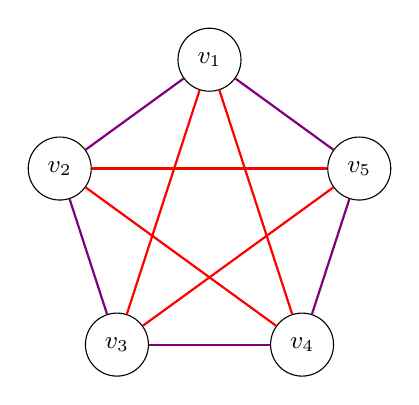
\begin{tikzpicture}[scale=2, every node/.style={circle, draw, minimum size=0.8cm, inner sep=1pt, font=\small}]

  % Vertices (pentagon layout)
  % these are polar coords. 90 means a right angle, 1 means the radius
  \node (v1) at (90:1)  {$v_1$};
  \node (v2) at (162:1) {$v_2$};
  \node (v3) at (234:1) {$v_3$};
  \node (v4) at (306:1) {$v_4$};
  \node (v5) at (18:1)  {$v_5$};

  % Purple C5 edges
  \draw[thick, purple] (v1) -- (v2);
  \draw[thick, purple] (v2) -- (v3);
  \draw[thick, purple] (v3) -- (v4);
  \draw[thick, purple] (v4) -- (v5);
  \draw[thick, purple] (v5) -- (v1);

  % Forced blue edges
  \draw[red, thick] (v1) -- (v3);
  \draw[red, thick] (v1) -- (v4);
  \draw[red, thick] (v2) -- (v5);
  \draw[red, thick] (v2) -- (v4);
  \draw[red, thick] (v3) -- (v5);

\end{tikzpicture}
\caption{The $K_5$ counterexample with the colouring described in the proof}
\end{figure}


\hfill$\blacksquare$
\section{Proving that $R(4,C_4)$ only contains one structurally unique counterexample (up to swapping of colours and relabeling of vertices):}
Proof: Suppose there is a complete graph with the vertices $v_1,v_2,v_3,v_4$, with the purple Hamiltonian cycle $v_1v_2,v_2v_3,v_3v_4,v_4v_1.$. It is worth noting that a relabeling of vertices would not change the core argument. Suppose that $v_1v_3$ and $v_2v_4$ are the same colour. This would form a monochromatic $K_4$. Therefore, by the pigeonhole principle, it can be assumed that there is one blue and one red edge. Further arguments using this $K_4$ as a subgraph can be made up to swapping, and would halve the number of required computations.\\

\begin{figure}[h!]
\centering
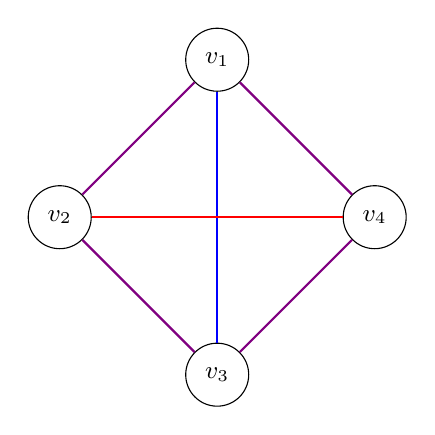
\begin{tikzpicture}[scale=2, every node/.style={circle, draw, minimum size=0.8cm, inner sep=1pt, font=\small}]
  % Vertices (pentagon layout)
  % these are polar coords. 90 means a right angle, 1 means the radius
  \node (v1) at (90:1)  {$v_1$};
  \node (v2) at (180:1) {$v_2$};
  \node (v3) at (270:1) {$v_3$};
  \node (v4) at (360:1) {$v_4$};
  % Purple C4 edges
  \draw[thick, purple] (v1) -- (v2);
  \draw[thick, purple] (v2) -- (v3);
  \draw[thick, purple] (v3) -- (v4);
  \draw[thick, purple] (v1) -- (v4);
  % Forced blue edges
  \draw[blue, thick] (v1) -- (v3);
  % Forced red edges
  \draw[red, thick] (v2) -- (v4);
\end{tikzpicture}
\caption{The $K_4$ counterexample with the colouring described in the proof}
\end{figure}
\hfill$\blacksquare$
\section{Proving that $R(4,C_4)>5$:}
Firstly, it is a necessity to prove that $R(4,C_4) > 5$. A counterexample for $K_5$ can be found below. 
\begin{figure}[h!]
\centering
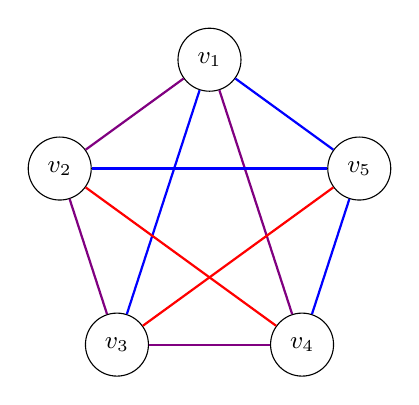
\begin{tikzpicture}[scale=2, every node/.style={circle, draw, minimum size=0.8cm, inner sep=1pt, font=\small}]
  % Vertices (pentagon layout)
  % these are polar coords. 90 means a right angle, 1 means the radius
  \node (v1) at (90:1)  {$v_1$};
  \node (v2) at (162:1) {$v_2$};
  \node (v3) at (234:1) {$v_3$};
  \node (v4) at (306:1) {$v_4$};
  \node (v5) at (18:1)  {$v_5$};

  % Purple C_4 edges
  \draw[thick, purple] (v1) -- (v2);
  \draw[thick, purple] (v2) -- (v3);
  \draw[thick, purple] (v3) -- (v4);
  \draw[thick, purple] (v1) -- (v4);

  % Forced blue edges
  \draw[blue, thick] (v1) -- (v3);
  \draw[blue, thick] (v2) -- (v5);
  \draw[blue, thick] (v1) -- (v5);
   \draw[blue, thick] (v4) -- (v5);

  % Forced red edges
  \draw[red, thick] (v2) -- (v4);
  \draw[red, thick] (v3) -- (v5);

\end{tikzpicture}
\caption{A $K_5$ counterexample. Please note this is not the only counterexample and non-isomorphic counterexamples do exist.}
\end{figure}
To find $R(4,C_4)$, it is essential to understand how counterexamples for $K_5$ were constructed. Firstly, a new vertex $v_5$ was added. Once again, we construct sets of edges which cannot all be a certain colour. At least one element of the set $\{v_1v_5,v_3v_5,v_4v_5\}$ must be blue, since we would otherwise have a blue $K_4$. Similarly, at least one element of the set $\{v_2v_5,v_3v_5,v_4v_5\}$ must be blue. The same principle can be applied to find that there is at least one red edge in the sets $\{v_1v_5,v_2v_5,v_3v_5\}$ and $\{v_2v_5,v_3v_5,v_4v_5\}$. It then logically follows that there is at least one red edge and one blue edge in the set. 
$\{v_1v_5,v_2v_5,v_3v_5,v_4v_5\}$.

%Now, suppose there is a new vertex $v_6$. Similarly, we find that the set 
%${v_1v_6,v_2v_6,v_3v_6,v_4v_6\}$ contains red and blue edges.

\hfill$\blacksquare$
\section{Proving that $R(4,C_5)$ only contains one structurally unique counterexample:}
Proof: We are trying to find a positive integer $n$ such that any $K_n$ with a purple $C_5$ subgraph would contain a blue $K_4$ or red $K_4$. This result will be verified computationally with a Julia program, but the uniqueness of the counterexample will be proved here. If we assume one counterexample for $K_5$ (up to relabeling and colour swapping), we can reduce the necessary computations by a factor of 32.\\


We will first define the smallest possible value for $n$ where this graph could exist. The smallest graph where a purple $C_5$ could exist is $K_5$. Let there be a $K_5$ with the vertices $v_1$, $v_2$, $v_3$, $v_4$, and $v_5$. We will now define a purple Hamilton 5-cycle with the edges

\\\centering $v_1v_2$, $v_2v_3$, $v_3v_4$, $v_4v_5$, $v_5v_1$\\
\begin{flushleft}
up to relabeling vertices. We can now apply the inclusion-exclusion principle. It is worth noting that any non-purple subset of the form with at least two adjacent purple edges can be analysed with the following method, and generality is therefore not lost when choosing edges. Suppose that $v_1v_3$,$v_1v_4$ and $v_2v_4$ are the same colour. This would lead to a monochromatic $K_4$. Therefore, by the pigeonhole principle, we know that two of these edges must be the same colour. Without loss of generality, (up to swapping and vertex relabeling) we will assume that $v_1v_4$ and $v_1v_3$ are blue. To avoid a blue $K_4$, $v_3v_5$ and $v_2v_4$ must now both be red. This forces $v_2v_5$ to be blue. Therefore, we can conclude, that up to relabeling of vertices and swapping of colours, the counterexample for $R(4,4,C_5)$ is unique. Even when we select different edges to colour, we still obtain isomorphisms of this counterexample. 
\end{flushleft}
% h is here, ! is to avoid LaTeX constraints

\begin{figure}[h!]
\centering
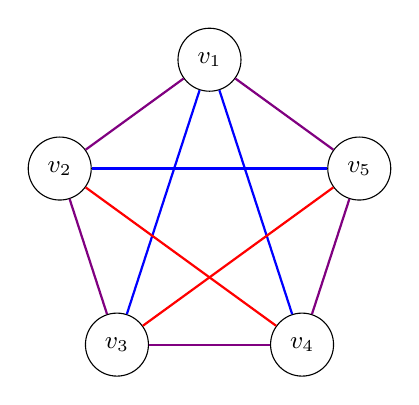
\begin{tikzpicture}[scale=2, every node/.style={circle, draw, minimum size=0.8cm, inner sep=1pt, font=\small}]
  % Vertices (pentagon layout)
  % these are polar coords. 90 means a right angle, 1 means the radius
  \node (v1) at (90:1)  {$v_1$};
  \node (v2) at (162:1) {$v_2$};
  \node (v3) at (234:1) {$v_3$};
  \node (v4) at (306:1) {$v_4$};
  \node (v5) at (18:1)  {$v_5$};

  % Purple C5 edges
  \draw[thick, purple] (v1) -- (v2);
  \draw[thick, purple] (v2) -- (v3);
  \draw[thick, purple] (v3) -- (v4);
  \draw[thick, purple] (v4) -- (v5);
  \draw[thick, purple] (v5) -- (v1);

  % Forced blue edges
  \draw[blue, thick] (v1) -- (v3);
  \draw[blue, thick] (v1) -- (v4);
  \draw[blue, thick] (v2) -- (v5);

  % Forced red edges
  \draw[red, thick] (v2) -- (v4);
  \draw[red, thick] (v3) -- (v5);

\end{tikzpicture}
\caption{The $K_5$ counterexample with the colouring described in the proof}
\end{figure}
\begin{flushleft}
If we assume $v_1v_4$ and $v_3v_5$ to be blue, $v_1v_3$ must be red. Notably, regardless of the colours chosen for $v_2v_4$ and $v_2v_5$, we find an isomorphism of the previous graph. If we make both edges red, we find the previous counterexample with swapped colours. Counterexamples where  one edge is assumed to be red and one edge is assumed to be blue, leads to an isomorphism of the previous counterexample with relabelling of vertices. It must be noted that both edges cannot be the same colour, because this would lead to a monochromatic $K_4$. This means that when adding vertices and exploring larger complete graphs with this constraint, such as $K_6$ and $K_7$, we can assume that this $K_5$ is a subgraph without loss of generality.
\end{flushleft}



\hfill$\blacksquare$

\end{document}
